% GNUPLOT: LaTeX picture with Postscript
\begingroup
  \makeatletter
  \providecommand\color[2][]{%
    \GenericError{(gnuplot) \space\space\space\@spaces}{%
      Package color not loaded in conjunction with
      terminal option `colourtext'%
    }{See the gnuplot documentation for explanation.%
    }{Either use 'blacktext' in gnuplot or load the package
      color.sty in LaTeX.}%
    \renewcommand\color[2][]{}%
  }%
  \providecommand\includegraphics[2][]{%
    \GenericError{(gnuplot) \space\space\space\@spaces}{%
      Package graphicx or graphics not loaded%
    }{See the gnuplot documentation for explanation.%
    }{The gnuplot epslatex terminal needs graphicx.sty or graphics.sty.}%
    \renewcommand\includegraphics[2][]{}%
  }%
  \providecommand\rotatebox[2]{#2}%
  \@ifundefined{ifGPcolor}{%
    \newif\ifGPcolor
    \GPcolorfalse
  }{}%
  \@ifundefined{ifGPblacktext}{%
    \newif\ifGPblacktext
    \GPblacktexttrue
  }{}%
  % define a \g@addto@macro without @ in the name:
  \let\gplgaddtomacro\g@addto@macro
  % define empty templates for all commands taking text:
  \gdef\gplbacktext{}%
  \gdef\gplfronttext{}%
  \makeatother
  \ifGPblacktext
    % no textcolor at all
    \def\colorrgb#1{}%
    \def\colorgray#1{}%
  \else
    % gray or color?
    \ifGPcolor
      \def\colorrgb#1{\color[rgb]{#1}}%
      \def\colorgray#1{\color[gray]{#1}}%
      \expandafter\def\csname LTw\endcsname{\color{white}}%
      \expandafter\def\csname LTb\endcsname{\color{black}}%
      \expandafter\def\csname LTa\endcsname{\color{black}}%
      \expandafter\def\csname LT0\endcsname{\color[rgb]{1,0,0}}%
      \expandafter\def\csname LT1\endcsname{\color[rgb]{0,1,0}}%
      \expandafter\def\csname LT2\endcsname{\color[rgb]{0,0,1}}%
      \expandafter\def\csname LT3\endcsname{\color[rgb]{1,0,1}}%
      \expandafter\def\csname LT4\endcsname{\color[rgb]{0,1,1}}%
      \expandafter\def\csname LT5\endcsname{\color[rgb]{1,1,0}}%
      \expandafter\def\csname LT6\endcsname{\color[rgb]{0,0,0}}%
      \expandafter\def\csname LT7\endcsname{\color[rgb]{1,0.3,0}}%
      \expandafter\def\csname LT8\endcsname{\color[rgb]{0.5,0.5,0.5}}%
    \else
      % gray
      \def\colorrgb#1{\color{black}}%
      \def\colorgray#1{\color[gray]{#1}}%
      \expandafter\def\csname LTw\endcsname{\color{white}}%
      \expandafter\def\csname LTb\endcsname{\color{black}}%
      \expandafter\def\csname LTa\endcsname{\color{black}}%
      \expandafter\def\csname LT0\endcsname{\color{black}}%
      \expandafter\def\csname LT1\endcsname{\color{black}}%
      \expandafter\def\csname LT2\endcsname{\color{black}}%
      \expandafter\def\csname LT3\endcsname{\color{black}}%
      \expandafter\def\csname LT4\endcsname{\color{black}}%
      \expandafter\def\csname LT5\endcsname{\color{black}}%
      \expandafter\def\csname LT6\endcsname{\color{black}}%
      \expandafter\def\csname LT7\endcsname{\color{black}}%
      \expandafter\def\csname LT8\endcsname{\color{black}}%
    \fi
  \fi
  \setlength{\unitlength}{0.0500bp}%
  \begin{picture}(10204.00,6802.00)%
    \gplgaddtomacro\gplbacktext{%
      \csname LTb\endcsname%
      \put(946,704){\makebox(0,0)[r]{\strut{} 0}}%
      \csname LTb\endcsname%
      \put(946,1390){\makebox(0,0)[r]{\strut{} 20}}%
      \csname LTb\endcsname%
      \put(946,2076){\makebox(0,0)[r]{\strut{} 40}}%
      \csname LTb\endcsname%
      \put(946,2763){\makebox(0,0)[r]{\strut{} 60}}%
      \csname LTb\endcsname%
      \put(946,3449){\makebox(0,0)[r]{\strut{} 80}}%
      \csname LTb\endcsname%
      \put(946,4135){\makebox(0,0)[r]{\strut{} 100}}%
      \csname LTb\endcsname%
      \put(946,4821){\makebox(0,0)[r]{\strut{} 120}}%
      \csname LTb\endcsname%
      \put(946,5508){\makebox(0,0)[r]{\strut{} 140}}%
      \csname LTb\endcsname%
      \put(946,6194){\makebox(0,0)[r]{\strut{} 160}}%
      \csname LTb\endcsname%
      \put(1078,484){\makebox(0,0){\strut{} 0}}%
      \csname LTb\endcsname%
      \put(2048,484){\makebox(0,0){\strut{} 0.05}}%
      \csname LTb\endcsname%
      \put(3018,484){\makebox(0,0){\strut{} 0.1}}%
      \csname LTb\endcsname%
      \put(3988,484){\makebox(0,0){\strut{} 0.15}}%
      \csname LTb\endcsname%
      \put(4958,484){\makebox(0,0){\strut{} 0.2}}%
      \csname LTb\endcsname%
      \put(5927,484){\makebox(0,0){\strut{} 0.25}}%
      \csname LTb\endcsname%
      \put(6897,484){\makebox(0,0){\strut{} 0.3}}%
      \csname LTb\endcsname%
      \put(7867,484){\makebox(0,0){\strut{} 0.35}}%
      \csname LTb\endcsname%
      \put(8837,484){\makebox(0,0){\strut{} 0.4}}%
      \csname LTb\endcsname%
      \put(9807,484){\makebox(0,0){\strut{} 0.45}}%
      \put(176,3620){\rotatebox{-270}{\makebox(0,0){\strut{}$U_H$ (\si{\milli\volt})}}}%
      \put(5442,154){\makebox(0,0){\strut{}$B$ (\si{\tesla})}}%
    }%
    \gplgaddtomacro\gplfronttext{%
      \csname LTb\endcsname%
      \put(3850,6278){\makebox(0,0)[r]{\strut{}$I_{12} = \SI{2.5}{\milli\ampere}$}}%
      \csname LTb\endcsname%
      \put(3850,5885){\makebox(0,0)[r]{\strut{}$U_H(\si{\milli\volt})=\num{223} \cdot B(\si{\tesla})$}}%
      \csname LTb\endcsname%
      \put(3850,5492){\makebox(0,0)[r]{\strut{}$I_{12} = \SI{5.0}{\milli\ampere}$}}%
      \csname LTb\endcsname%
      \put(3850,5099){\makebox(0,0)[r]{\strut{}$U_H(\si{\milli\volt})=\num{420} \cdot B(\si{\tesla})$}}%
    }%
    \gplbacktext
    \put(0,0){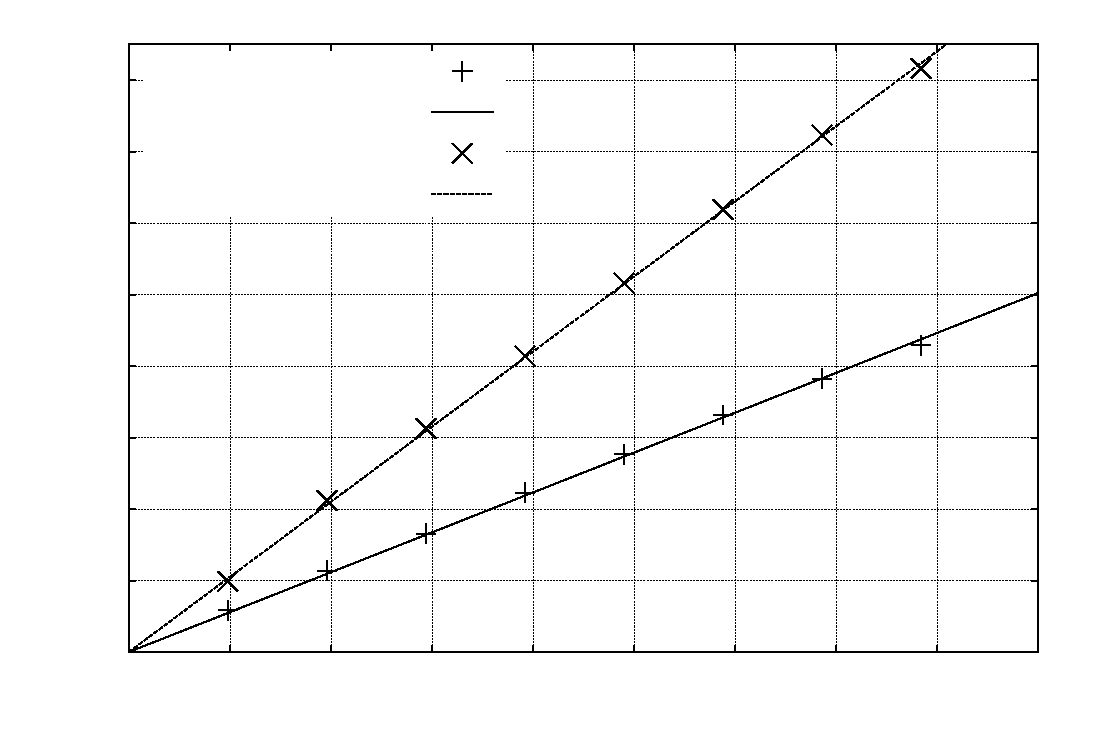
\includegraphics{hall}}%
    \gplfronttext
  \end{picture}%
\endgroup
